\kap{Computational Methods}\label{chap:Coputational Methods}

This chapter is devoted to computational calculations. Most of the theoretical equations are
explained in other chapters. Numerical methods for
calculating the bound state energy of the deuteron and the scattering problem
for a two nucleon system, given an already made potential,  are discussed throughly.

Calculations of binding energy can be done both from the \LS ${}$ equation and the \SE. Only the \SE${}$ 
method will be shown. For the phase shift calculations results will be given both in bar formalism and 
Blatt-Biedenharn formalism. These are the most common definitions of phase shift for coupled channels.
One method Thompson has recommended over the more used \LS ${}$ equation, is also included.
Computers were slow in beginning of such numerical calculations, this led to the use of the R-matrix. 
The R-matrix works for low energy problems where a non complex potential is used, and is a approximation
of the T-matrix.

Kowalski recommended a method which he published in 1965 (REF). This method use a mathematical method 
which is equivalent to the \LS ${}$ equation. In this method the singularity in the propagator, is introduced later
in the calculations. These methods are compared.

Note that it is often smart to do a quick dimensional check of the equations before one use the equations in a computer program.
This way one can detect errors in an early phase, and save time. 

%\begin{flushleft}




\section{Calculating NN-Binding Energy in Deuteron} 

For a bound state $\ket{\psi_B}$ we have $E<0$. To find the binding energy, we need to find the eigenvalues of the
$\SE$. If we use relative coordinates. From (\ref{eq:senterofmass}) we have
\begin{equation}
\bigg[-\frac{1}{2\mu} {\bf \triangledown}^2+V({\bf r}) \bigg]\psi({\bf r})=E_{}\psi({\bf r})
\end{equation}
If a Fourier transformation into momentum space is done , we get
\begin{equation}
\frac{k^2}{2\mu}\psi({ k})+\frac{2}{\pi}\int^\infty_0 dp\;p^2 V({ k},{ p})\psi({ p})=E_{}\psi_({ k})  
\end{equation}
This integral can be calculated numerically using Gaussian quadrature. In this approach we introduce $N$, which is
the number of fixed lattice points. The integral can then be approximated by $N$ weights $\omega_i$ and $N$ mesh points $x_i$.
\begin{equation}
\frac{k^2}{2\mu}\psi({ k})+\frac{2}{\pi}\sum^N_{i=1}\omega_i\;p^2_i  V({ k},{ p_i})\psi({ p_i})=E_{}\psi({ k})
\end{equation}

Theoretically one would expect an error in this equation to be smaller if $N$ is increased. Numerically this isn't necessary
the truth,
since the sum can create round off error that blows up if the biggest numbers cancel each other.

If we choose $k=p_j$ we have N-equations, and N-unknown eigenvalues. We can rewrite it as a matrix equation,
\begin{equation}\label{eq:egen}
H{\Psi}=E{\Psi}
\end{equation}

Where
\begin{equation}
{\Psi}=
\left( \begin{array}{c}
{\psi}(p_1)\\
{\psi}(p_2)\\
\vdots\\
{\psi}(p_N)
\end{array}\right)
\end{equation}
And

\begin{equation}
H_{ij}={p_{j}^2}{2\mu}+\frac{2}{\pi}\sum^N_{i=1}\omega_i;p^2_i  V({ p_j},{ p_i})\psi({ p_i})
\end{equation}

From (\ref{eq:egen}) we will get N-eigenvalues, but only the negative values will be eigenvalues of bound states. i.e. 
binding energies. 

In my program, I solve the integral with the Gauss-Legendre method called gauleg. This gives weights $w_i$ and mesh points $x_i$.
$x_i$ will be
in the interval $[-1,1]$. Since the integral goes from $0$ to $\infty$, we need to map these weights and mesh points. This mapping
can be done with the tan function 
%to respectively $\omega$ and $p_i\in [0,\infty]$ by using the tan-mapping give
\begin{equation}
p_i=C\tan\bigg(\frac{\pi}{4}(1+x_i)\bigg)
\end{equation}
If we derivate this equation for the new mesh points and multiply it with the old weights, we get the new weights
\begin{equation}
\omega_i=C\frac{\pi}{4}\frac{w_i}{\cos ^2\big(\frac{\pi}{4}(1+x_i)\big)}
\end{equation}

$C$ is  a constant, and in our case $C=1000$ seems to be good choice. 
%$C$ determines how the mesh points are distributed after the mapping. Half the mesh points will be less than $C$,
%and the other half will be greater than $C$.

The eigenvalues are calculated using an IMSL function called DEVLCG. This returns the eigenvalues in decreasing order for a general
Hermittian matrix.

If one use the Bonn B potential, the coupled channel case potential should be defined as

\begin{equation}
V=
\left( \begin{array}{cc}
V(3) & V(5)\\
V(6) & V(4)
\end{array}\right)
=
\left( \begin{array}{cc}
\braketm{l=j+1}{V}{l'=j+1} & \braketm{l=j+1}{V}{l'=j-1}\\
\braketm{l=j-1}{V}{l'=j+1} & \braketm{l=j-1}{V}{l'=j-1}
\end{array}\right)
\end{equation}

Where $V(i)$ is the potential returned from the Bonn B
%This can of course also be read from the $\LS$ equation, where we use we insert a complete set of states for both positive
%and negative energies, so that
%\begin{equation}
%\inv{E-\op{H}\pm i\epsilon}=\sum_N\frac{\ket{\varphi_n}\bra{\varphi_n}}{E-E_n}
%+\frac{1}{(2\pi)^3}\int^\infty_{-\infty}d^3q\frac{\ket{\varphi_q}\bra{\varphi_q}}{E-E_q\pm i\epsilon}
%\end{equation}


We only get one bound state using the Bonn B potential at an energy of $-2.2246$ MeV.
This is for the \state{3}{S}{1}. This state is only possible for a 
proton-neutron system, and the bound state is known as the deuteron. 
The experimental value of the binding energy is $2.224575$  MeV
\footnote{From C. van der Leun and C. Alderlisten, Nucl. Phys A380, 261 (1982)}
, which is almost exactly what we got!\nl

This can of course also be read from the $\LS$ equation, where we use we insert a complete set of states for both positive
and negative energies, so that
\begin{equation}
\inv{E-\op{H}\pm i\epsilon}=\sum_N\frac{\ket{\varphi_n}\bra{\varphi_n}}{E-E_n}
+\frac{1}{(2\pi)^3}\int^\infty_{-\infty}d^3q\frac{\ket{\varphi_q}\bra{\varphi_q}}{E-E_q\pm i\epsilon}
\end{equation}

Where we removed the regulator for the bond states, since we have no pole for negative total energy ($E<0$). 

This $E_n$ is of course the bound states. The other eigenvalues we find are different $E_q$'s from the continuous 
specter with $E>0$.








\section{Solving With Minimal Relativity} 
My program can calculate the T-matrix in two different ways. We now solve the one called "Minimal Relativity", 
which has the form of the $\LS$ equations.
%"Minimal Relativity" which is exactly on the form 
as the $\LS$ equation. 
The other method is the the one called Thompson and is handled in the next section.
%This is the $\LS$ equation with  relativistic energies in the propagator.
These equations are related differently to the S-matrix. All of this is  explained in chapter (?????).
We now go back to (\ref{eq:Trelllll}) and look at the Minimal Relativity. 
%The Thompson case will be similar.
\begin{eqnarray}\label{eq:Trellllla}
\braketm{{ p}} {\op{T}_l(E_{ k})}{{ k}}&=&\braketm{{ p}}{\op{V}_l}{{ k}}
+ \frac{2m}{\pi}\;{\cal P}\int^{\infty}_{0}d { q}\; q^2 \quad\bra{{ p}}\op{V}_l\ket{{ q}}
\;\inv{{ k^2}-{ q^2}}   \;\bra{{ q}} \op{T}_l(E_{ k})\;\ket{{ k}}\nonumber\\
&&
-i { k}m \bra{{ p}}\op{V_l}\ket{{ k}}\bra{{ k}}
\;\bra{{ k}}\op{T}_l(E_{ k})\;\ket{{ k}}
\end{eqnarray}

To solve the integral, we use a trick where a constant is added in the integral. 
Noting that
\begin{equation}
{\cal }\int^{\infty}_{-\infty}\frac{d q}{k-{ q}}=0
\end{equation}
we get
\begin{equation}
{\cal }\int^{\infty}_{-\infty}\frac{d q}{k-{ q}}
=
{\cal }\int^{\infty}_{0}\frac{d q}{k-{ q}}+{\cal }\int^{0}_{-\infty}\frac{d q}{k-{ q}}
=
2k{\cal }\int^{\infty}_{0}\frac{d q}{k^2-{ q^2}}=0
\end{equation}


So that we can add 0 by adding
\begin{equation}\label{eq:trix0}
-\frac{2m}{\pi}\;k^2\bra{{ p}}\op{V}_l\ket{{ k}}    
\bra{{ k}} \op{T}_l(E_{ k})\;\ket{{ k}}\;{\cal }\int^{\infty}_{0}\frac{d q}{k^2-{ q^2}}=0
\end{equation}


This constant will remove the singularity. And if we 
don't have any singularities, we can as well remove ${\cal P}$. We have 
\begin{eqnarray}\label{eq:Trelllllaa}
\braketm{{ p}} {\op{T}_l}{{ k}}&=&\braketm{{ p}}{\op{V}_l}{{ k}}
+ \frac{2m}{\pi}\int^{\infty}_{0}d { q}
\inv{{ k^2}-{ q^2}}\bigg[ q^2\bra{{ p}}\op{V}_l\ket{{ q}} \bra{{ q}} \op{T}_l\ket{{ k}}\nonumber\\
&&-
k^2\bra{{ p}}\op{V}_l\ket{{ k}}
\bra{{ k}} \op{T}_l\ket{{ k}}\bigg]
-i { k}m \bra{{ p}}\op{V_l}\ket{{ k}}
\bra{{ k}}\op{T}_l\ket{{ k}}
\end{eqnarray}

This is now a smooth integral, and we can compute it like we did in the last section. Where we used Gauss-Legendre with a remaping
of the mesh points so that the new mesh points are in the interval $[0,\infty]$. 
We then have mesh points
\begin{equation}
q_i=C\tan\bigg(\frac{\pi}{4}(1+x_i)\bigg)
\end{equation}
and weights
\begin{equation}
\omega_i=C\frac{\pi}{4}\frac{w_i}{\cos ^2\big(\frac{\pi}{4}(1+x_i)\big)}
\end{equation}
Where $x_i$ and $w_i$ are respectively the mesh points and the weights from Gauss-Legendre. $C$ should be chosen around 1000MeV. 
Then, this mapping is optimal
for calculating this problem. i.e. we need less mesh points to get the same accuracy. Since half the mesh points will are
than $C$, the integral accuracy will be relatively good in this region $[0 MeV,1000 MeV]$ where the integrand can vary a lot.   

We can now rewrite (\ref{eq:Trelllllaa})
\begin{eqnarray}\label{eq:Trelllllaae}
\braketm{{ p}}{\op{V}_l}{{ k}}&=&\braketm{{ p}} {\op{T}_l}{{ k}}
- \frac{2m}{\pi}\sum^N_{j=1}
\frac{\omega_j q^2_j}{{ k^2}-{ q^2_j}}\bra{{ p}}\op{V}_l\ket{{ q_j}} \bra{{ q_j}} \op{T}_l\ket{{ k}}\nonumber\\
&&+
\frac{2m}{\pi}\bra{{ p}}\op{V}_l\ket{{ k}}
\bra{{ k}} \op{T}_l\ket{{ k}}\sum^N_{j=1} \frac{\omega_jk^2}{{ k^2}-{ q^2_j}}
-
i { k}m \bra{{ p}}\op{V_l}\ket{{ k}}
\bra{{ k}}\op{T}_l\ket{{ k}}
\end{eqnarray}

Let us first look at the  uncoupled states, and deal with the coupled  states later. 
The singlet and triplet states have $N$ unknowns contained in $\braketm{{ q_i}} {\op{T}_l}{{ k}}$ $+$ one unknown from
$\bra{{ k}}\op{T}_l\ket{{ k}}$, but we only have $N$ equations. To be able to solve the problem we 
define $q_{N+1}=k$, where $k$ is the on-shell momentum 
and let $p$ have all the values $q_i$ .e.i. $1\le i\le(N+1)$.
We can now solve the problem because we have
$(N+1)$ unknowns in $\braketm{{ q_i}} {\op{T}_l}{{k}}$ and we have $(N+1)$ equations!
Rewriting (\ref{eq:Trelllllaae}) we only have to solve the matrix equation
\begin{equation}\label{eq:AT=V} 
AT=V
\end{equation}
Now $A$ is a $(N+1)\times (N+1)$ matrix defined as
\begin{equation}
A_{i,j}=\delta_{i,j}-\braketm{{ q_i}} {\op{V}_l}{{ q_j}} u_j
\end{equation}
Where $\delta$ is the Kronecker delta, and $u$ is a $(N+1)$ vector defined as
\begin{equation}\label{eq:uj1}
u_j=\frac{2m}{\pi}\frac{\omega_jq^2_j}{q^2_{N+1}-{ q^2_j}}\qquad\textrm{for $1\le j\le N$}
\end{equation}
and
\begin{equation}\label{eq:ujN1}
u_{N+1}=-\frac{2m}{\pi}\sum^N_{j=1}\frac{\omega_jq^2_{N+1}}{{ q^2_{N+1}}-{ q^2_j}}+  im q_{N+1}
\end{equation}

We see that if $V$ is known, so are $A$. From (\ref{eq:AT=V}) we then have all we need to calculate
the unknown $T$. Multiplying the inverse $A$-matrix ($A^{-1}$) from the left hand side of (\ref{eq:AT=V}), we have
\begin{equation}\label{eq:T=AinvV}
T=A^{-1}V
\end{equation}

To calculate the inverse of a matrix I use the IMSL call DLINCG. This function returns the inverse matrix of any complex matrix.

Having found the on-shell T-matrix, we are able to calculate the S-matrix. From (\ref{eq:Sl2}) we have
\begin{equation}\label{eq:S_lMR}
S_l =1-2imk\; T_{N+1,N+1}
\end{equation}

And from the S-matrix we have the phase shifts and inelasticities(\ref{eq:deltaski}).
\begin{equation}
\eta_l\; e^{2i\delta_l}=S_l=|S_l|\;\exp\bigg(i\;\tan^{-1}\bigg[\frac{{\cal I}m\{S_l\}}{{\cal R}e\{S_l\}}\bigg]\bigg)
\end{equation}
So we have
\begin{equation}
\eta_l=|S_l|
\end{equation}
\begin{equation}
{\delta_l}=\frac{1}{2}\tan^{-1}\bigg(\frac{{\cal I}m\{S_l\}}{{\cal R}e\{S_l\}}\bigg)
\end{equation}
\nl
For couplet channels we have to do things a little bit differently. First of all we define a new
$2(N+1)\times 2(N+1)$ potential matrix $V_c$. We use the notation "$+$" for $l=j+1$, and "$-$" for $l=j-1$.
So if $V_{l,l'}=V_{+-}$, it means $\braketm{l=j+1}{V}{l'=j-1}$
\begin{equation}
V_c=
%\left( \begin{array}{cc}
%V(3) & V(5)\\
%V(6) & V(4)
%\end{array}\right)
%=
\left( \begin{array}{cc}
\braketm{q_i}{V_{++}}{q_j} & \braketm{q_i}{V_{+-}}{q_j}\\
\braketm{q_i}{V_{-+}}{q_j} & \braketm{q_i}{V_{--}}{q_j}
\end{array}\right)
\end{equation}

and defining a $2(N+1)\times 2(N+1)$ matrix $A_c$
\begin{equation} 
A_c=
\left( \begin{array}{rr}
\delta_{i,j}-\braketm{q_i}{V_{++}}{q_j} u_j & -\braketm{q_i}{V_{+-}}{q_j}u_j \\
-\braketm{q_i}{V_{-+}}{q_j} u_j             &\quad \delta_{i,j} -\braketm{q_i}{V_{--}}{q_j}u_j
%-u_j\quad \braketm{l=j+1}{V}{l'=j+1} \quad +\delta_{i,j} & -u_j \braketm{l=j+1}{V}{l'=j-1}\\
%-u_j\quad \braketm{l=j-1}{V}{l'=j+1}                     & -u_j \braketm{l=j-1}{V}{l'=j-1}\quad  
\end{array}\right)
\end{equation}

Where $u_j$ and $q$ are the same as before. By taking the inverse of $A_c$, we can determine the $2(N+1)\times 2(N+1)$
T-matrix. Since we just need the on-shell elements of the T-matrix to calculate the S-matrix, we only calculate the
$2\times 2$-matrix
\begin{equation}\label{eq:SuperSmatrisen}
\left(
\begin{array}{cc} {{ \op{S}^{J1}_{++} }}
&
{ \op{S}^{J1}_{+-} } \\
 \op{S}^{J1}_{-+}
&
 \op{S}^{J1}_{--}
\end{array} \right)
=
\left(
\begin{array}{cc}
1 & 0\\
0 &1
\end{array} \right) 
-imk\; 
\left( \begin{array}{cc}
\braketm{q_{N+1}}{T_{++}}{q_{N+1}} & \braketm{q_{N+1}}{T_{+-}}{q_{N+1}} \\
\braketm{q_{N+1}}{T_{-+}}{q_{N+1}} & \braketm{q_{N+1}}{T_{--}}{q_{N+1}}
\end{array}\right)
\end{equation}

Finding phase shifts, inelasticities and the mixing factor in "Blatt-Biedenharn"- or "bar"- formalism,
is then straight forward. All the formulas needed
are given in (\ref{eq:bar-eps}) - (\ref{eq:Blatt-tre}).
\nl
This method can cause trouble for big N, i.e. large number of mesh points. 
The propagator will blow up when we choose mesh points close to $q_{N+1}$. 
Since we used the trick to to add a "zero"-term to remove the singularity in the integrand, 
we can loose numerical precision. 
%so the two terms will cancel each other in the region of the singularity.
Numerically we will loose precision when we add and subtract large numbers that cancel each other. 
One can expect such errors to enter when mesh points gets close to the singularity. 
These errors have to go through a matrix
inversion and a matrix multiplication.  This problem turns out to be small. Even with $N=600$ the result is good. 
To avoid this problem I have implemented a function in my program that can determine when a mesh point is "to close"
to $q_{N+1}$. It is possible to avoid some of these "problems" by using a method by Kowalski. Where the singularity is removed in the last step,
with the same zero-term trick. This way we don't blow up an error during other calculations. These errors turn out to be extremely small. 
Even for $N=600$ the difference between the methods is of order $10^{-12}$.    





\section{Solving With "Thompson"} 
The only difference in solving the Thompson equation instead of the Minimal Relativity equation, will be
in the $u_j$ and in the relation between $S_l$ and $T_l$. The potential $V$ will of course be different, 
since the two methods are based upon different approaches. 
The Thompson and "Minimal relativity" are two different approximations from the Bethe-Salpeter equation.
These two approaches has different propagators in the Lippmann-Scwinger equation. This will lead to different
relations between the S and T matrix in the two cases. Also the constant we add to numerical 
solve an integral with a singularity will be affected.
With Thompson the $u_j$ in (\ref{eq:uj1}) - (\ref{eq:ujN1}) will changed to
\begin{equation}
u_j=\frac{\omega_jq^2_j}{\pi}\;\bigg(\frac{\sqrt{q^2_j+m^2}+\sqrt{q^2_{N+1}+m^2}}{q^2_{N+1}-{ q^2_j}}\bigg)\qquad\textrm{for $1\le j\le N$}
\end{equation}
and
\begin{equation}
u_{N+1}=-\frac{2}{\pi}\sum^N_{j=1}\frac{\omega_jq^2_{N+1}\sqrt{q^2_{N+1}+m^2}}{{ q^2_{N+1}}-{ q^2_j}}+  i q_{N+1}\sqrt{q^2_{N+1}+m^2}
\end{equation}
Also (\ref{eq:S_lMR}) will be updated to 
\begin{equation}
S_l =1-i2q_{N+1}\;\sqrt{q^2_{N+1}+m^2}\; T_{N+1,N+1}
\end{equation}
For coupled channels, the similar equation
\begin{equation}
\left(
\begin{array}{cc} {{ \op{S}^{J1}_{++} }}
&
{ \op{S}^{J1}_{+-} } \\
\op{S}^{J1}_{-+}
&
\op{S}^{J1}_{--}
\end{array} \right)
=
\left(
\begin{array}{cc}
1 & 0\\
0 &1
\end{array} \right)
-iq_{N+1}\;\sqrt{q^2_{N+1}+m^2}\;
\left( \begin{array}{cc}
{T_{++}} &{T_{+-}} \\
{T_{-+}} &{T_{--}}
\end{array}\right)
\end{equation}
Will replace (\ref{eq:SuperSmatrisen}).
Using the Thompson method with Kowalski equations are similar done.







\section{The R-Matrix}
Sometimes it is preferable to calculate the R-matrix, also known as the "K-matrix" instead of using the T-matrix.
The R-matrix is a simplifying T-matrix. To derive it one need to use the optical theorem 
or it's related $\op{T}_l$ in the center of mass system (\ref{eq:bevisT246}) is given as:
\begin{eqnarray}\label{eq:bevisTferd}
{\cal I}\textrm{m}\bigg\{\braketm{{ k}}{\op{T}_l}{{ k}}\bigg\}=
- m k |\braketm{{   k}}{\op{T}_l}{{ k}}|^2
\end{eqnarray}
We are interested in defining a practical $\op{R}$ which is real, but still obey some of the similar relations as $\op{T}$. We now
split the real part of the T-matrix, so we have ${\cal R}e\{\op{T}_l\}=\op{R}_l-iimk\op{r}_l$ where both $\op{R}_l$ and $\op{r}_l$ are real. 
The on shell T-matrix can be written as
\begin{eqnarray}\label{eq:R-matrisanesten}
\braketm{{   k}}{\op{T}_l}{{ k}} &=& \braketm{{   k}}{\op{R}_l}{{ k}} +{\cal I}\textrm{m} \bigg\{\braketm{{   k}}{\op{T}_l}{{ k}}\bigg\}
-iimk\braketm{{   k}}{\op{r}_l}{{ k}}\nonumber\\
&=&
\braketm{{   k}}{\op{R}_l}{{ k}}  -imk\bigg(|\braketm{{   k}}{\op{T}_l}{{ k}}|^2 +i\braketm{{   k}}{\op{r}_l}{{ k}}\bigg)\nonumber\\
&=&
\braketm{{   k}}{\op{R}_l}{{ k}}  -imk\bigg(\braketm{{   k}}{\op{T}_l}{{ k}}^\dagger +i\frac{\braketm{{   k}}{\op{r}_l}{{ k}}}
{\braketm{{   k}}{\op{T}_l}{{ k}}}\bigg)\braketm{{   k}}{\op{T}_l}{{ k}}\nonumber\\
&\equiv&
\braketm{{   k}}{\op{R}_l}{{ k}}  -imk\braketm{{   k}}{\op{R}_l}{{ k}}\braketm{{   k}}{\op{T}_l}{{ k}}
%-i\pi R\delta(E-\op{H}_0)T %=R-i\frac{m}{k}\delta(q-k)RT
\end{eqnarray}
Where we in the last step defined the on shell R-matrix in partial waves.%, by choosing a value for $\braketm{{   k}}{\op{r}_l}{{ k}}$.
Subtracting (\ref{eq:R-matrisanesten}) with its complex conjugate
\begin{eqnarray}\label{eq:bevisTferd1}
{\op{R}_l}-{\op{R}_l}^\dagger=\big(\op{T}_l-\op{T}^\dagger_l\big)+ ir_l \frac{\op{T}^\dagger_l+\op{T}_l}{\op{T}^\dagger_l\op{T}_l}\doteq 0
\end{eqnarray}
%Where we have used that $R_l$ is real.
From this equation it is possible define a real $\op{R}_l$-matrix, by choosing a real $\op{r}_l$ 
%so that satisfies (\ref{eq:bevisTferd1}). 
%By choosing this $\op{r}_l$, we also define $\op{R}_l$.\nl
%
Defining the R-matrixes off-shell elements the same way as T, 
will lead the R-matrix to obey the same $\LS$ equation as T did! But since R is real it will only contain 
the real parts of the $\LS$ equation. Therefor it will only work for real potentials, i.e. total elastic scattering.
% So for R we have (\ref{eq:Trelllllaheyiy})
%The last step in (\ref{eq:R-matrisanesten}) is possible because both $R_l$ and $r_l$ are real, so
%\begin{eqnarray}\label{eq:bevisTferd1}
%{\op{R}_l}-{\op{R}_l}^\dagger=\big(T_l-T^\dagger_l\big)+ ir_l \frac{T^\dagger_l+T_l}{T^\dagger_lT_l}\doteq 0
%\end{eqnarray}
%We see that it is possible to choose a real $\op{r}_l$ so that this equation is satisfied. By choosing this $\op{r}_l$, we also
%define $\op{R}_l$.
%
In operator form the R-matrix is defined as
\begin{equation}\label{eq:R-matrisa}
\op{T}\equiv \op{R}-i\pi \op{R}\delta(E-\op{H}_0)\op{T} %=R-i\frac{m}{k}\delta(q-k)RT
\end{equation}
%
%
%This definition is chosen so that $\op{R}$ is real, and therefor it will only work for real potentials, i.e. total elastic scattering.
the R-matrix  will make the program much faster, since all the matrix equations are now real instead of complex. The R-matrix
has been widely used  before, but since an accurate calculation of the on-shell 
T-matrix are done within seconds. It's not a "must" anymore.
For example if one use the Bonn B potential, going from 
T-matrix calculations to R-matrix, one will not even make the program twice as fast! 
%Because R is real, it can not contain information about a complex potential.

The rate in which we save time by using the R-matrix is also dependent on the potential. If we use a real potential, the
time to make the potential matrix $V_l(p,k)$ will be approximately the same, i.e.
%time it takes for the potential to be calculated.
%This time will be the same for the T-matrix as the R-matrix, and 
it will be of order $N\times N\times$ ("number of operations done in
the potential") while a real matrix inversion will be of order $N^3$. If one use a simple potential as the box potential, we see that
we save more time (relative to T) using the R-matrix.

We will probably see more people "going back" to the more general T-matrix in the future. 
Because we use more and more time consuming potentials. Today the low energy region, where we can use the R-matrix, 
is very well simulated. While the more high
energy potentials are still to be developed.\nl
%
From (\ref{eq:bevisTferd1}) a similar minimal relativity equation (\ref{eq:Trellllla}) for the complex R-matrix, can be obtained.
(GAA IGJENNOM DETTE EN GANG TIL)
\begin{eqnarray}\label{eq:Trelllllaheyiy}
\braketm{{ p}} {\op{R}_l}{{ k}}&=&\braketm{{ p}}{\op{V}_l}{{ k}}
+ \frac{2m}{\pi}\;{\cal P}\int^{\infty}_{0}d { q}\; q^2\;\bra{{ p}}\op{V}_l\ket{{ q}}
\;\inv{{ k^2}-{ q^2}}   \;\bra{{ q}} \op{R}_l\;\ket{{ k}}
\end{eqnarray}
We note that in (\ref{eq:TsomTme}) we had that
\begin{equation}
2imk\;\bra{k}\op{T}_{l}\;\ket{{ k}}=1-e^{2i\delta_l}=e^{i\delta_l}\Big(e^{-i\delta_l}-e^{i\delta_l}\Big)
\end{equation}
The phase shifts for the spin singlet can be found by inserting this $T_l$ in (\ref{eq:R-matrisanesten} ). 

We then arrive for the spin singlet
\begin{equation}\label{eq:deltasfasing}
\tan {\;}^0\delta^J(\textrm{T}_{lab})=-\;2km{\;}^0R^J(k,k)
\end{equation}
and uncoupled spin triplet
\begin{equation}\label{eq:deltasfatrip}
\tan {\;}^1\delta^J(\textrm{T}_{lab})=-\;2km{\;}^1R^J(k,k)
\end{equation}
Using the Blatt and Biedenharn convention for the coupled states, we have
\begin{equation}\label{eq:deltasfacob}
\tan \bar{\delta}^J_\mp(\textrm{T}_{lab})=-\frac{1}{2}km\bigg[R^J_{--}+R^J_{++}\pm\frac{R^J_{--}+R^J_{++}}
{\cos(2\bar{\epsilon}_J)}\bigg]
\end{equation}
\begin{equation}\label{eq:taneps}
\tan\bigg(2\bar{\epsilon}_J(\textrm{T}_{lab})\bigg)=\frac{2R^J_{+-}}{R^J_{--}-R^J_{++}}
\end{equation}
Where $\bar{\epsilon}$ is the mixing factor.














\section{The Kowalski method}
The Kowalski method
~\cite{Kowalski}
%\footnote{K. L. Kowalski, Phys. Rev. Lett. 15 798 (1965)}
is a method where we rewrite the $\LS$ equation, so that we can delay the introduction of the singularity.
We now look at the minimal relativity case. From (\ref{eq:Trellllla}) we have
\begin{equation}\label{eq:Tmy11}
\braketm{{ p}} {\op{T}_l}{{ k}} =\braketm{{ p}}{\op{V}_l}{{ k}}
+ \frac{2m}{\pi}{\cal P}\int^{\infty}_{0}d { q}\; q^2 \frac{\bra{{ p}}\op{V}_l\ket{{ q}}}
{k^2- q^2}  \bra{{ q}} \op{T}_l\ket{{ k}}
-i { k}m \bra{{ p}}\op{V_l}\ket{{ k}}\bra{{ k}}\op{T}_l\ket{{ k}}  
\end{equation}
From this equation we also have
\begin{eqnarray}\label{eq:Tmy12}
\frac{\braketm{ p}{\op{V}_l}{ k} }{\braketm{ k}{\op{V}_l}{ k} }\braketm{ k}{\op{T}_l}{ k} 
&=&
\braketm{{ p}}{\op{V}_l}{{ k}}
+ \frac{2m}{\pi}{\cal P}\int^{\infty}_{0}d { q}\; q^2
\frac{\bra{{ p}}\op{V}_l\ket{{ k}}\braketm{{ k}}{\op{V}_l}{{ q}} }{\braketm{{ k}}{\op{V}_l}{{ k}} } 
\inv{k^2- q^2}  \bra{{ q}} \op{T}_l\ket{{ k}}\nonumber\\
&&
-i { k}m \bra{{ p}}\op{V_l}\ket{{ k}}\bra{{ k}}\op{T}_l\ket{{ k}}  
\end{eqnarray}
Subtracting (\ref{eq:Tmy12}) from (\ref{eq:Tmy11}), we have
\begin{eqnarray}\label{eq:Tmy113}
\braketm{{ p}} {\op{T}_l(E)}{{ k}} &=&
\frac{\braketm{ p}{\op{V}_l}{ k} }{\braketm{ k}{\op{V}_l}{ k} }\braketm{ k}{\op{T}_l(E)}{ k}\\%\nonumber\\ 
&&
+ \frac{2}{\pi}\int^{\infty}_{0}d { q}\; q^2 \bigg[\bra{{ p}}\op{V}_l\ket{{ q}}-
\frac{\bra{{ p}}\op{V}_l\ket{{ k}}\braketm{{ k}}{\op{V}_l}{{ q}} }{\braketm{{ k}}{\op{V}_l}{{ k}} }\bigg] 
\inv{{k^2- q^2}}  \bra{{ q}} \;\op{T}_l(E)\;\ket{{ k}}\nonumber
\end{eqnarray}
Where we have removed the principal value ${\cal P}$, since there are no singularities in this integral.
%To calculate this we can do as before, 
The integral is calculated by using a remaping of  the Gauss-Legendre mesh points
to the interval $[0,\infty]$. We let $p$ have all the values $q_i$ for $1\le i\le N$
\begin{eqnarray}\label{eq:Tmy1134}
\braketm{{ q_i}} {\op{T}_l(E)}{{ k}} &=&
\frac{\braketm{ q_i}{\op{V}_l}{ k} }{\braketm{ k}{\op{V}_l}{ k} }\braketm{ k}{\op{T}_l(E)}{ k}%\nonumber\\
+ \frac{2m}{\pi}\sum^N_{j=1}\omega_j q^2_j \bigg[\bra{{ q_i}}\op{V}_l\ket{{{ q}_j}}\nonumber\\
&&
-\frac{\bra{{ q_i}}\op{V}_l\ket{{ k}}\braketm{{ k}}{\op{V}_l}{{ q_j}} }{\braketm{{ k}}{\op{V}_l}{{ k}} }\bigg]
\inv{ k^2-{{ q^2}_j}}  \bra{{ q_j}} \;\op{T}_l(E)\;\ket{{ k}}%\nonumber
\end{eqnarray}
We now have $N+1$ unknowns and $N$ equations. 
To solve this equations, we divide (\ref{eq:Tmy1134}) by $\braketm{ k}{\op{T}_l(E)}{ k}$.
We will then only have $N$ unknowns with respect to $\braketm{{ q_i}} {\op{T}_l(E)}{{ k}}/\braketm{ k}{\op{T}_l(E)}{ k}$.
%So it will be possible to solve (\ref{eq:Tmy1134}), we have
\begin{eqnarray}\label{eq:Tmy11345}
\frac{\braketm{{ q_i}} {\op{T}_l(E)}{{ k}}}{\braketm{ k}{\op{T}_l(E)}{ k}} &=&
\frac{\braketm{ q_i}{\op{V}_l}{k} }{\braketm{ k}{\op{V}_l}{ k }}
+ \frac{2m}{\pi}\sum^N_{j=1}\frac{\omega_j q^2_j}{(k^2- q^2_j)} \bigg[\bra{{ q_i}}\op{V}_l\ket{{{ q}_j}}\nonumber\\
&&
-\frac{\bra{{ q_i}}\op{V}_l\ket{{ k}}\braketm{{k}}{\op{V}_l}{{ q_j}} }{\braketm{{ k}}{\op{V}_l}{{k}} }\bigg]
\frac{\bra{{ q_j}} \;
\op{T}_l(E)\;\ket{{ k}}}{\braketm{ k}{\op{T}_l(E)}{ k}}%\nonumber
\end{eqnarray}
To find the unknown ${\braketm{ k}{\op{T}_l(E)}{ k}}$, we go back to the $\LS$ equation  
(\ref{eq:Tmy11}), and substitute
\begin{equation}
{\braketm{{ q_i}} {\op{T}_l(E)}{{ k}}}
=
\frac{\braketm{{ q_i}} {\op{T}_l(E)}{{ k}}}{\braketm{ k}{\op{T}_l(E)}{ k}}{\braketm{ k}{\op{T}_l(E)}{ k}} 
\end{equation}
By doing this, the singularity will enter the equation again. This singularity can be handled 
as before, where we added a zero term (\ref{eq:trix0}) that removes the singularity in the integrand.
Finally we let $p=k$, and we obtain
\begin{equation}\label{eq:Tmy113456} 
{\braketm{ k}{\op{T}_l}{ k}}
=
\frac{\braketm{{k}}{\op{V}_l}{{ k}} }
{1-\frac{2m}{\pi}\sum_{j=1}^N \frac{\omega_j}{ k^2- q^2_j}
\bigg[q^2_j\braketm{{ k}}{\op{V}_l}{{ q_j}}
\frac{\braketm{{ q_j}} {\op{T}_l}{{ k}}}{\braketm{ k}{\op{T}_l}{ k}}
-{ k^2\braketm{{ k}}{\op{V}_l}{{ k}}} \bigg]
+
i { k}m \bra{{ k}}\op{V_l}\ket{{ k}}    }
\end{equation}
We see that this equation have two terms with singularities  that cancel each other.
As mentioned before. This can give numerical loss in precision for mesh points close to $k$, and cause an error. This error
will generally increase with $N$, because more points will be close to the singularity. 
%like we had using the other method. 
%This method can cause problems if a mesh point is getting too close
%to $q_{N+1}$. The reason for this is that the Gauss-Legendre method doesn't 
%give a good result if one of the mesh points is to  close to a singularity.
%Since the method are based on polynomial (of degree 2N-1) approximation of the original integrand. 
%But if we increase
%Because the propagator term will blow up. Since  
A good guess though is that this method will be better than the other one for large $N$, because the main numerical errors are introduced late, 
and errors are more likely to grow if they are introduced early.
\nl
To calculate (\ref{eq:Tmy11345}) we can build up a matrix equation
\begin{equation}
T=B^{-1}U
\end{equation}
Where $B$ is a $N\times N$ matrix, and both $T$ and $U$ are arrays of length $N$ 
\begin{equation}
T_i=\frac{\braketm{{ q_i}} {\op{T}_l}{{ k}}}{\braketm{ k}{\op{T}_l}{ k}} 
\end{equation}
\begin{equation}
U_{i}=\frac{\braketm{ q_i}{\op{V}_l}{ k} }{\braketm{ k}{\op{V}_l}{k} }
\end{equation}
\begin{equation}
B_{i,j}=\delta_{i,j}-
\bigg[\bra{{ q_i}}\op{V}_l\ket{{{ q}_j}}-U_{i}{\braketm{{ k}}{\op{V}_l}{{ q_j}} }\bigg]q^2_j s_j
\end{equation}
Where  
\begin{equation}
s_j=\frac{2m}{\pi} \frac{\omega_j}{k^2-{ q^2_j}}  \qquad\textrm{for $1\le j\le N$}
\end{equation}
%\begin{equation}
%v_j=\frac{2m}{\pi}\frac{\omega_jq^2_j}{k^2-{ q^2_j}}  \qquad\textrm{for $1\le j\le N$}   
%\end{equation}
So when the $T$-array is calculated, we can find $\bra{{ k}}\op{T_l}\ket{{ k}}$ from (\ref{eq:Tmy113456})
\begin{equation}
\bra{{ k}}\op{T_l}\ket{{ k}}
=\frac{\bra{k}\op{V}_l\ket{k}}{1+\sum_{j=1}^N\bigg[q^2_j\bra{k}\op{V}_l\ket{q_j}T_j-k^2\braketm{ k}{\op{V}_l}{k} \bigg] s_j
+i { k}m \bra{{ k}}\op{V_l}\ket{{ k}}} 
\end{equation}
This equation is calculated straight forward. 
%When we now have found $\bra{{ k}}\op{T_l}\ket{{ k}}$. 
We can use the same methods as before
to calculate the phase shifts from the known$\bra{{ k}}\op{T_l}\ket{{ k}}$!
\nl
If we compare this method (Kowalski) with the method used before from "Brown and Jackson". We find the results from 
the two methods very similar. It also turns out that for my code the "Brown and Jackson" method is only about 1$\%$ faster 
than the Kowalski method. This difference is really too small to recommend one method over the other.
Maybe the difference would be different if one used a simpler
potential than the Bonn B potential. 

The similarities of the two methods can be seen in the table below. Where phase shift for \state{1}{S}{0} 
with lab energy 25MeV
are solved (with the minimal relativity) for the Bonn B potential are shown. % %(\ref{tab:sammenlikningKow&Brown}) 
The phase shifts are given with 14 digits after comma. 
This high precision is interesting when analyzing numerical methods, but
doesn't make  physical sense. Since the Bonn B potential is build up of
theories and parameters of much less precision.
\nl
\begin{flushleft}
\begin{table}
\begin{tabular}{|l|c|c|c|c|c|c|}%\label{tab:sammenlikningKow&Brown}
\hline
N&  (A)(B)(C)  &  \multicolumn{2}{|c|}{Kowalski}  & \multicolumn{2}{|c|}{Brown and Jackson} & Difference  \\
\hline
            &          &  Phase shift & time              &       Phase shift    &  time       & Phase shift    \\
\hline
3           &(0)(0)(0) &   71.62345689430250 & 0.04s      & 71.62345689430260    & 0.04s       & 1.0E-13       \\
\hline
5           &(0)(0)(0) &   41.46263918236210 & 0.05s      & 41.46263918236210    & 0.05s       & 0            \\
\hline
10          &(0)(0)(0) &   51.08156285146330 & 0.17s      & 51.08156285146330    & 0.15s       & 0            \\
\hline
25          &(1)(0)(0) &   50.71696055173802 & 0.90s      & 50.71696055173803    & 0.89s       & 1.0E-14          \\ 
\hline
50          &(0)(0)(0) &   50.71674962783273 & 3.09s      & 50.71674962783273    & 3.09s       & 0        \\
\hline
75          &(0)(0)(0) &   50.71674749296322 & 7.11s      & 50.71674749296330    & 7.00s       & 8.0E-14     \\
\hline
100         &(0)(0)(0) &   50.71674746062610 & 14.32s     & 50.71674746062610    & 13.55s      & 0            \\
\hline
150         &(2)(0)(0) &   50.71674746145212 &     --     & 50.71674746145210    &     --      & 2.0E-14        \\
\hline
200         &(0)(0)(0) &   50.71674745769040 &     --     & 50.71674745769050    &     --      & 1.0E-13        \\
\hline
250         &(0)(0)(0) &   50.71674745807750 &     --     & 50.71674745807711    &     --      & 3.9E-13        \\
\hline
300         &(1)(0)(0) &   50.71674745539690 &     --     & 50.71674745539662    &     --      & 2.8E-13      \\
\hline
350         &(1)(0)(0) &   50.71674745671981 &     --     & 50.71674745671972    &     --      & 1.1E-13        \\
\hline
400         &(1)(0)(0) &   50.71674746084243 &     --     & 50.71674746084244    &     --      & 1.0E-14      \\
\hline
450         &(2)(0)(0) &   50.71674745973450 &     --     & 50.71674745973450    &     --      & 0        \\
\hline
500         &(1)(0)(0) &   50.71674745780814 &     --     & 50.71674745780800    &     --      & 1.4E-13      \\
\hline
550         &(1)(0)(0) &   50.71674745755723 &     --     & 50.71674745755700    &     --      & 2.3E-13        \\
\hline
600         &(3)(0)(0)*&   50.71674745788354 & 1266s      & 50.71674745788430    & 1257s       & 7.6E-13        \\ 
\hline
650         &(0)(0)(0) &   50.71674745747293 &     --     & 50.71674745747272    &     --      & 2.1E-13      \\
\hline
700         &(3)(0)(0)*&   50.71674745725370 &     --     & 50.71674745725340    &     --      & 3.0E-13     \\
\hline
750         &(1)(0)(0) &   50.71674745849564 &     --     & 50.71674745849570    &     --      & 6.0E-14    \\
\hline
800         &(0)(0)(0) &   50.71674745901132 &     --     & 50.71674745783083    &     --      & 1.2E-9      \\
\hline
850         &(1)(0)(0) &   50.71674745774120 &     --     & 50.71674745774120    &     --      & 0      \\
\hline
\hline
789         &p(3)(1)(1)&  50.71674745784843 &   2727s     & 50.71674745784860    & 2624s       & 1.7E-13      \\
\hline
801         &(1)(0)(0) &  50.71674745781930 &      --     & 50.71674745781930    &     --      & 0      \\
\hline
802         &(2)(0)(0) &  50.71674745762290 &      --     & 50.71674745762272    &     --      & 2.8E-13      \\
\hline
803         &(2)(0)(0) &  50.71674745783440 &      --     & 50.71674745783370    &     --      & 7.0E-13      \\
\hline
821         &p(0)(0)(0)&  50.71674745783100 &   3352s     & 50.71674745783083    &  3182s      & 1.7E-13      \\
\hline
843         &p(3)(2)(0)*& 50.71674746936084 &      --     & 50.71674747021500    &     --      & 8.5E-10      \\
\hline
\end{tabular}
\caption{
\label{tabKowalskysammenlikning}
Accuracy and computer running time using two different numerical methods to calculate the phase shifts.
}
\end{table}
\end{flushleft}
%\nl
Where (A) is number of mesh points ($q_i$) in the region $q_{N+1}\pm 5.0$E-2 MeV,
(B) in the region $q_{N+1}\pm5.0$E-3 MeV and (C) in the  region $q_{N+1}\pm 5.0$E-4 MeV.
The time is the time used to run the program which calculates the phase shift for 15 different lab energies.

"*" Denotes the cases where the S-matrix is not exactly unitary for the standard method (Brown and Jackson).
The Kowalski method on the other hand, is unitary in those cases. By coincident, it also happens for the Kowalski
method. The errors are small. Biggest inelasticity error observed was 5.0E-14. 

"p" Denotes that the mesh points where specially picked due to its interesting configuration of mesh points, but
not how the difference in phase shift.
All
the other mesh points are picked randomly with respect to $q_{N+1}$
\nl
Note that  numerical errors in the phase shift calculations are expected to be totally random. 
From the table~\ref{tabKowalskysammenlikning} a good estimate
of the phase shift will be 50.7167474578, which has 12 counting digits.
With this in mind, the number of correct reproduced digits for the rest of the phase shifts 
have bin plotted in fig~\ref{figtellenesiffeta}.
\begin{flushleft}
\begin{figure}
\centering
\includegraphics[height=15cm,angle=-90]{tellenesiffet.eps}
\caption{\label{figtellenesiffeta} Phase shifts in table~\ref{tabKowalskysammenlikning} 
are compared with a 12 digit phase shift which is
believed to be numerical correct.}
\end{figure}

%\newpage
%fig~\ref{fig:tellenesiffet}: Phase shifts in table ??? are compared with a 12 digit phase shift which is 
%believed to be numerical exact. 
\end{flushleft}



With mesh points less than 30, it seems like the difference between the phase shifts for the two methods
is less than 1.0E-13. It looks like the difference is slowly increasing with the number of mesh points. Which
is probably due to more numerical errors. Since the number of calculations done are increasing rapidly with N ($\sim N^3$). 
For 600 mesh points, when calculated for 15 different lab energies, the difference was found to be less than 1.0E-12. 
With N=843 the difference was in the order of 1.0E-7. 

Numerical errors can be divided into two parts. One due to the
to the accuracy in the integral calculation. This error will usually be less as N increase, and will depend on the potential.
The other part is due to the error all the numerical roundoff
errors will make, and this will be more or less independent of the potential. This error will, statistically, increase with N.
If we assume that the two methods generate independent errors, then the difference in the phase shifts will give us information
about the size of the numerical roundoff errors. 

The cases where the difference is 0, we clearly see that the assumption of independent roundoff errors
isn't always very good. For some mathematical-numerical reason "0" will turn up, even at large N.
To get the best estimate of the size of the error one should therefor study
each N with many energy-samples.
%But looking at other energies for the NN-interaction. In these cases, 
%we see that they are only statistical fenomenons*. 
%For some mathematical-numerical reason "0" will turn up, even at large N.
%At N=400 we have the first possible numerical roundoff error in order of 1.0E-8, but since the error is big
%compared with the phase shift difference, it is probably due to integral approximation errors.
In the table, the first obvious roundoff errors acoures in the Kowalski method for N=800. In this case
we have no mesh points close to $(q_{N+1})$. It is not the case it was created for. The normal method
gives very good result, and we clearly see the numerical round off errors acoures in the phase shifts. 
For N=843 both methods are involving
large round off errors. In this case there are two mesh points in the range of $(q_{N+1})\pm$1.0E-3. This is a situation
Kowalski had in mind when he recommended his method, and it is interesting to see that Kowalski was the best method in this case.

These errors doesn't
always acoures as big. It looks statistical like if something goes wrong, then a lot more will go wrong 
(Which is one of Murphys laws). 
But this doesn't happen to often (I believe Murphys laws never have proven to be correct, even though most of us experience different). 
For example $800\le N\le 850$ about 25$\%$ where such cases where the roundoff error blows up.
%Also the importance of a mesh point hitting close to the singularity seems to be small.

At N=789 there was one mesh point in the range of $(q_{N+1})\pm$1.0E-4. This was the only one one I could find in more than
a hundred tests. I was a little bit excited about how Kowalski would handle it. It did very well, but so did
the normal method. Both managed to reproduce the 12 first digits of the phase shift.
So the importance of a mesh point hitting close to the singularity seems to be small.

In summary the phase shifts in table~\ref{tabKowalskysammenlikning}  and fig~\ref{figtellenesiffeta} illustrates the facts:
\begin{itemize}
\item These methods are not only mathematically
equivalent, they are almost numerical identical to! With the Bonn Potential, one can trust about  
7 digits after the comma using mesh point between 200 and 600. But N=60 is good enough used on most potentials
on the marked today.
\item One should be careful using a large N (especially for N larger than 700), since this can reproduce
large numerical errors. If one need to find a higher precision of the phase shift,
one can look at an average of many samples with different N.
Or one can choose variables with better precision 
in the computer program, i.e. better than double precision.
\item Mesh points ending up as close as 5.0E-4 MeV to the singularity in the propagator seems to be of less importance
for the precision.
\item The methods use almost the same time.
\end{itemize}
 

These methods are almost numerical identical, and it is really hard to recommend one method over the other. 
Looks like Kowalski  was a little bit to worried about the numerical errors. The same can be said about Brown and Jackson.
In their book "Nucleon-Nucleon interaction" they also recommend the Kowalski method. Kowalski developed this
method in 1965. When Brown and Jackson recommended it in their book written in 1976,
computers that could handle more than a 100 mesh points didn't exist. And they would  not know if the problem was relevant
or not in real calculations.







%\end{flushleft} 
